\documentclass[12pt,a4paper]{article}
\usepackage[utf8]{inputenc}
\usepackage[english]{babel}
%\usepackage{minted}
\usepackage{listings}
\usepackage{xcolor}
\usepackage{graphicx}
\usepackage{geometry}
 \geometry{
 a4paper,
 total={170mm,257mm},
 left=25mm,
 top=20mm,
 right=25mm,
 bottom=20mm
 }

\title{\bf 8 Bit Arithmetic Operations}
\author{\vspace{-10ex}}
\date{\vspace{-10ex}}
\begin{document}
\maketitle

\begin{minipage}{0.45\textwidth}
        \begin{tabular}{l l}
            \textbf{Expt No:}&1\\
            \textbf{Date :}&21/08/2020
        \end{tabular}
\end{minipage}%
\begin{minipage}{0.45\textwidth}
        \begin{tabular}{l l}
             \textbf{Name:}& Shivanirudh S G  \\
             \textbf{Reg No:} & 185001146 
        \end{tabular}
\end{minipage}
\vspace{1cm}
\hrule
\begin{flushleft}
\subsection*{\textbf{Aim:}} 
To perform arithmetic operations on two 8 bit numbers.

\subsection*{\textbf{Procedure:}}
\begin{itemize}
    \item Mount masm folder to a drive on DOSBOX.
    \item Go to mounted drive.
    \item Save 8086 program with the extension \textbf{``.asm"} in the same folder using the command \textbf{``edit"}.
    \item Assemble the \textbf{.asm} file using the command \textbf{``masm filename.asm"}.
    \item Link the assmebled \textbf{.obj} file using the command \textbf{``link filename.obj"}.
    \item Debug the executable file \textbf{.exe} with the \textbf{``debug filename.exe"} command.
    \begin{itemize}
        \item The unassembled code can be viewed by the command \textbf{``u"}.
        \item Use the command \textbf{``d segment:offset"} to view the contents of memory locations from the specified segment:offset address.
        \item Use command \textbf{``e segment:offset"} to change the values in memory.
        \item Execute the program using command \textbf{``g"}.
        \item The command \textbf{``q"} exits from the debug session.
    \end{itemize}
\end{itemize}

\noindent\rule{\textwidth}{1.5pt}
\hrule
\newpage
\subsection*{\textbf{\underline{8 Bit Addition}}}

\subsubsection*{\textbf{Algorithm:}}
\begin{itemize}
    \item Move the data segment to the AX register and then move it to the DS register.
    \item Move the first operand to AH register. 
    \item Move the second operand to the BH register. 
    \item Initially set the CH register to 00h. 
    \item Then add using ADD AH,BH.
    \item Using JNC instruction check for carry and if there is no carry, no need to increment CH.
    \item Else, increment CH by 1. 
    \item The result and carry stored in AH and CH should be moved to RESULT
and CARRY respectively.
\end{itemize}

\newpage
\subsubsection*{\textbf{Program:}}

\begin{table}[htb]
\centering
\resizebox{\columnwidth}{!}{
\begin{tabular}{|l|l|} 
\hline
\textbf{Program}                                                 & \textbf{Comments}                             \\ 
\hline
\hline
assume cs:code,ds:data                                           & Declare code and data segments                \\
\hline
data segment                                                     & Start of data segment                         \\
\hline 
opr1 db 11h                                                      & Define byte opr1 with hex value 11            \\
\hline
opr2 db 99h                                                      & Define byte opr2 with hex value 99            \\
\hline
result db 00H                                                    & Define byte result with hex value 00          \\
\hline
carry db 00H                                                     & Define byte carry with hex value 00           \\
\hline      
data ends                                                        & End of data segment                           \\
\hline
code segment                                                     & Start of code segment                         \\
\hline
org 0100h                                                        & Set preferred offset                          \\
\hline
start:~ mov ax,data                                              & Move data segment contents to AX register     \\ 
\hline
mov ds,ax                                                        & Move data in AX register to DS register       \\ 
\hline
mov ah,opr1                                                      & Move contents of opr1 to AH register          \\ 
\hline
mov bh,opr2                                                      & Move contents of opr2 to BH register          \\ 
\hline
mov ch,00h                                                       & Move hex value 00 to CH register              \\ 
\hline
add ah,bh                                                        & AH = AH + BH                                  \\ 
\hline
jnc here                                                         & Jump to the label here, if there is no carry  \\ 
\hline
inc ch                                                           & Increment value of CH if there is a carry     \\ 
\hline
here:~ mov result,ah                                             & Move contents of AH register to result        \\ 
\hline
mov carry,ch                                                     & Move contents of CH register to carry         \\ 
\hline
int 21h                                                          & Request interrupt routine                     \\ 
\hline
code ends                                                        & End of code segment                           \\
\hline
end start                                                        &                                               \\
\hline
\end{tabular}
}
\end{table}

\newpage
\subsubsection*{\textbf{Input and Output:}}
\begin{figure}[h]
    \centering
    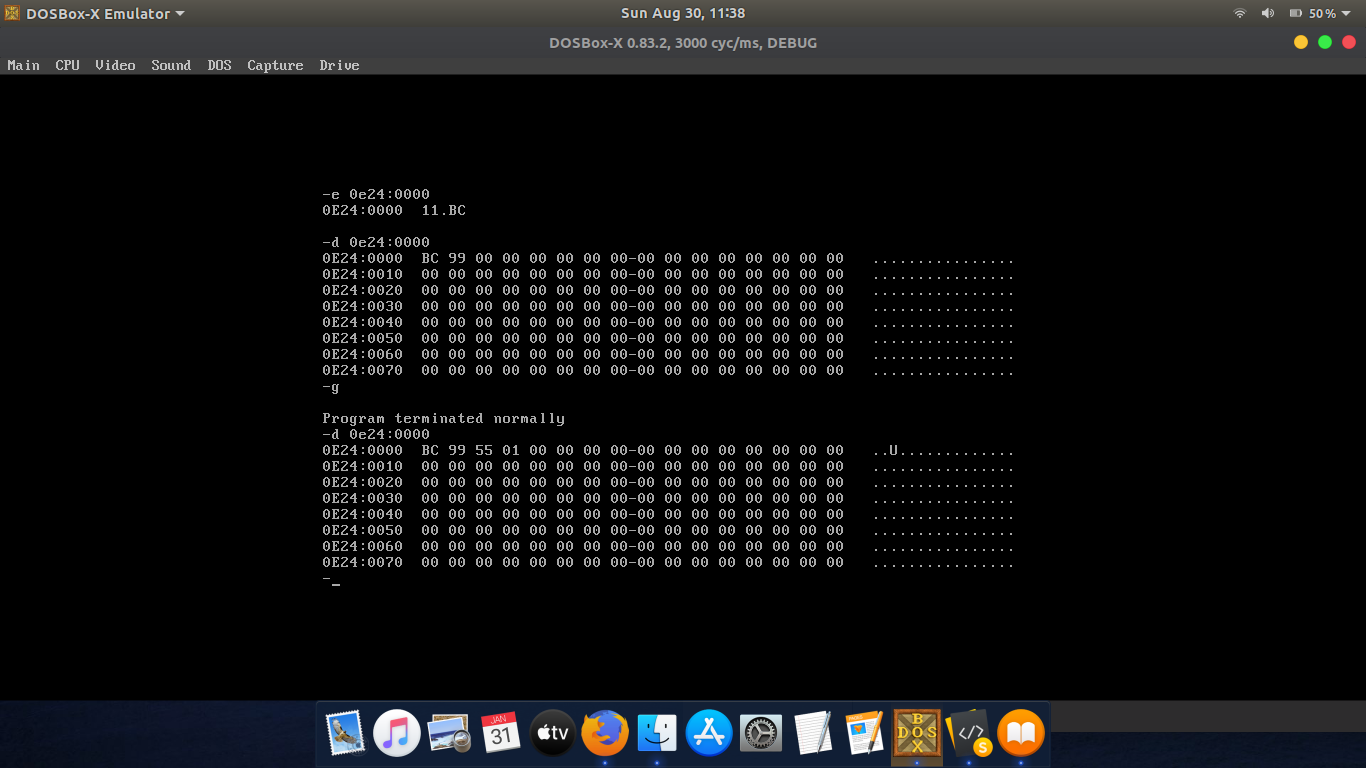
\includegraphics[trim = 100mm 70mm 100mm 80mm, clip, width = \textwidth]{Pics/Addition.png}
    \caption{ \textbf{Input:} \emph{opr1:} BCh, \emph{opr2:} 99h; 
              \textbf{Output:} \emph{Result:} 55h, \emph{Carry:} 01h}
\end{figure}
%----------------------------------------------------------------------------------------------------------------------------------------
\newpage
\subsection*{\textbf{\underline{8 Bit Subtraction}}}

\subsubsection*{\textbf{Algorithm:}}
\begin{itemize}
    \item Move the data segment to the AX register and then move it to the DS register.
    \item Move the first operand to AH register.
    \item Move the second operand to the BH register.
    \item Initially set the CH register to 00h.
\item Then subtract using SUB AH,BH.
\item Check for carry using JNC instruction. If no carry then it means AH $>$ BH and hence no need to increment CH and no need to complement AH.
\item Else, AH$<$BH. Hence we have to take 2’s complement of AH using NEG AH and also increment CH by 1 using INC CH.
\item The result and carry stored in AH and CH should be moved to RESULT and CARRY respectively.
\end{itemize}

\newpage
\subsubsection*{\textbf{Program:}}
\begin{table}[htb]
\centering\small
\resizebox{\columnwidth}{!}{
\begin{tabular}{|l|l|} 
\hline
\textbf{Program}                                                 & \textbf{Comments}                             \\ 
\hline
\hline
assume cs:code,ds:data                                           & Declare code and data segments                \\
\hline
data segment                                                     & Start of data segment                         \\
\hline 
opr1 db 11h                                                      & Define byte opr1 with hex value 11            \\
\hline
opr2 db 99h                                                      & Define byte opr2 with hex value 99            \\
\hline
result db 00H                                                    & Define byte result with hex value 00          \\
\hline
carry db 00H                                                     & Define byte carry with hex value 00           \\
\hline      
data ends                                                        & End of data segment                           \\
\hline
code segment                                                     & Start of code segment                         \\
\hline
org 0100h                                                        & Set preferred offset                          \\
\hline
start:~ mov ax,data                                              & Move data segment contents to AX register     \\ 
\hline
mov ds,ax                                                        & Move data in AX register to DS register       \\ 
\hline
mov ah,opr1                                                      & Move contents of opr1 to AH register          \\ 
\hline
mov bh,opr2                                                      & Move contents of opr2 to BH register          \\ 
\hline
mov ch,00h                                                       & Move hex value 00 to CH register              \\ 
\hline
sub ah,bh                                                        & AH = AH - BH                                  \\ 
\hline
jnc here                                                         & Jump to the label here, if there is no carry  \\ 
\hline
inc ch                                                           & Increment value of CH if there is a carry     \\ 
\hline
neg ah                                                           & Negate the contents of the AH register        \\
\hline
here:~ mov result,ah                                             & Move contents of AH register to result        \\ 
\hline
mov carry,ch                                                     & Move contents of CH register to carry         \\ 
\hline
int 21h                                                          & Request interrupt routine                     \\ 
\hline
code ends                                                        & End of code segment                           \\
\hline
end start                                                        &                                               \\
\hline
\end{tabular}
}
\end{table}

\newpage
\subsubsection*{\textbf{Input and Output:}}
\begin{figure}[h]
    \centering
    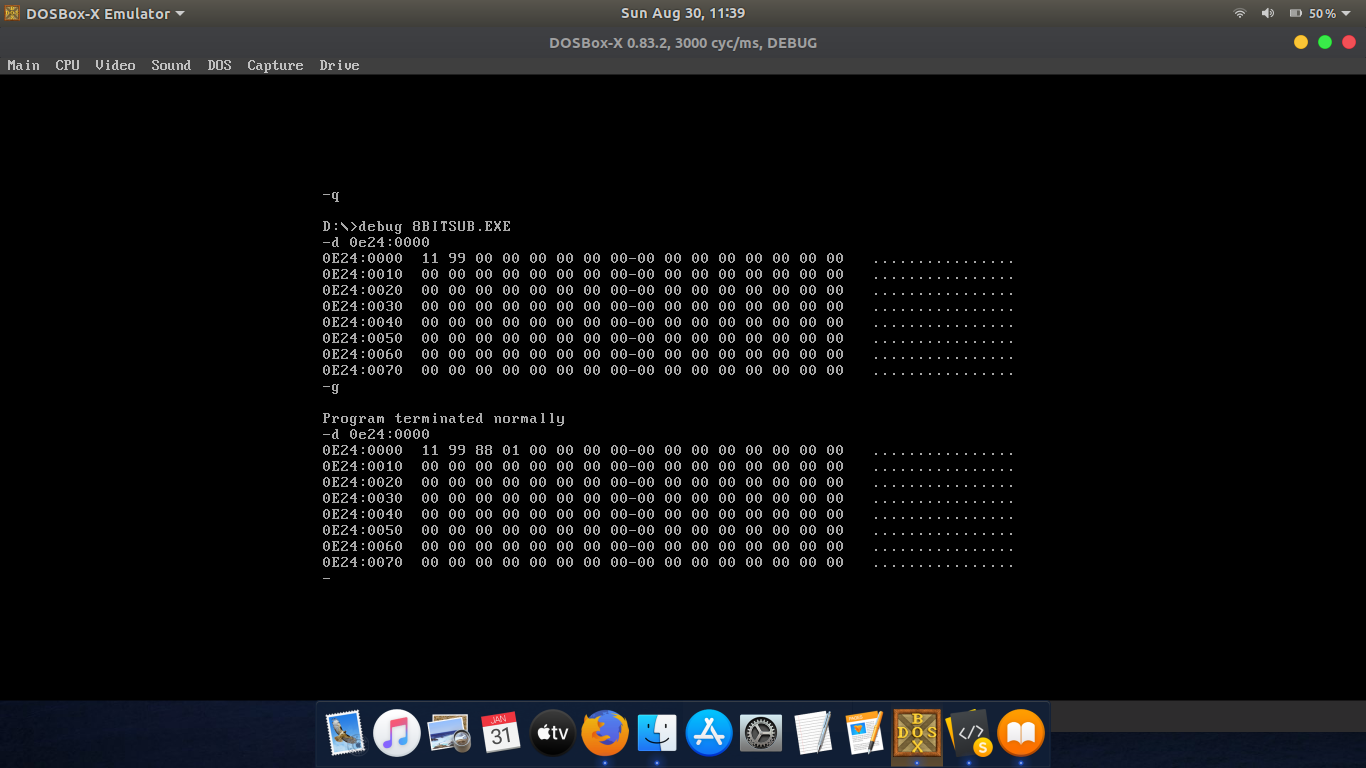
\includegraphics[trim = 100mm 70mm 100mm 80mm, clip, width = \textwidth]{Pics/Subtraction.png}
    \caption{ \textbf{Input:} \emph{opr1:} 11h, \emph{opr2:} 99h; 
              \textbf{Output:} \emph{Result:} 88h, \emph{Sign:} 01h}
\end{figure}


%----------------------------------------------------------------------------------------------------------------------------------------
\newpage
\subsection*{\textbf{\underline{8 Bit Multiplication}}}

\subsubsection*{\textbf{Algorithm:}}
\begin{itemize}
    \item Move the data segment to the AX register and then move it to the DS register.
    \item Move the first operand to AL register.
\item  Move the second operand to the BL register.
\item  Then multiply using MUL BL.(Since AL is default operand register for MUL instruction we only need to specify the other operand register.)
\item  The result stored in AX register(16 bit- because multiplication of two 8 bit numbers yields a 16 bit number) should now be moved to
RESULT.
\end{itemize}

\subsubsection*{\textbf{Program:}}
\begin{table}[htb]
\centering\small
\resizebox{\columnwidth}{!}{
\begin{tabular}{|l|l|} 
\hline
\textbf{Program}                                                 & \textbf{Comments}                             \\ 
\hline
\hline
assume cs:code,ds:data                                           & Declare code and data segments                \\
\hline
data segment                                                     & Start of data segment                         \\
\hline 
opr1 db 11h                                                      & Define byte opr1 with hex value 11            \\
\hline
opr2 db 99h                                                      & Define byte opr2 with hex value 99            \\
\hline
resulth db 00H                                                   & Define byte resulth with hex value 00         \\
\hline
resultl db 00H                                                   & Define byte resultl with hex value 00         \\
\hline      
data ends                                                        & End of data segment                           \\
\hline
code segment                                                     & Start of code segment                         \\
\hline
org 0100h                                                        & Set preferred offset                          \\
\hline
start:~ mov ax,data                                              & Move data segment contents to AX register     \\ 
\hline
mov ds,ax                                                        & Move data in AX register to DS register       \\ 
\hline
mov al,opr1                                                      & Move contents of opr1 to AL register          \\ 
\hline
mov ah, 00H                                                      & Move hex value 00 to AH register              \\
\hline
mov bh,opr2                                                      & Move contents of opr2 to BH register          \\ 
\hline
mul bh                                                           & AX = AL * BH                                  \\ 
\hline
here:~ mov resulth,ah                                            & Move contents of AH register to resulth       \\ 
\hline
mov resultl,al                                                   & Move contents of AL register to resultl       \\ 
\hline
int 21h                                                          & Request interrupt routine                     \\ 
\hline
code ends                                                        & End of code segment                           \\
\hline
end start                                                        &                                               \\
\hline
\end{tabular}
}
\end{table}

\newpage
\subsubsection*{\textbf{Input and Output:}}
\begin{figure}[h]
    \centering
    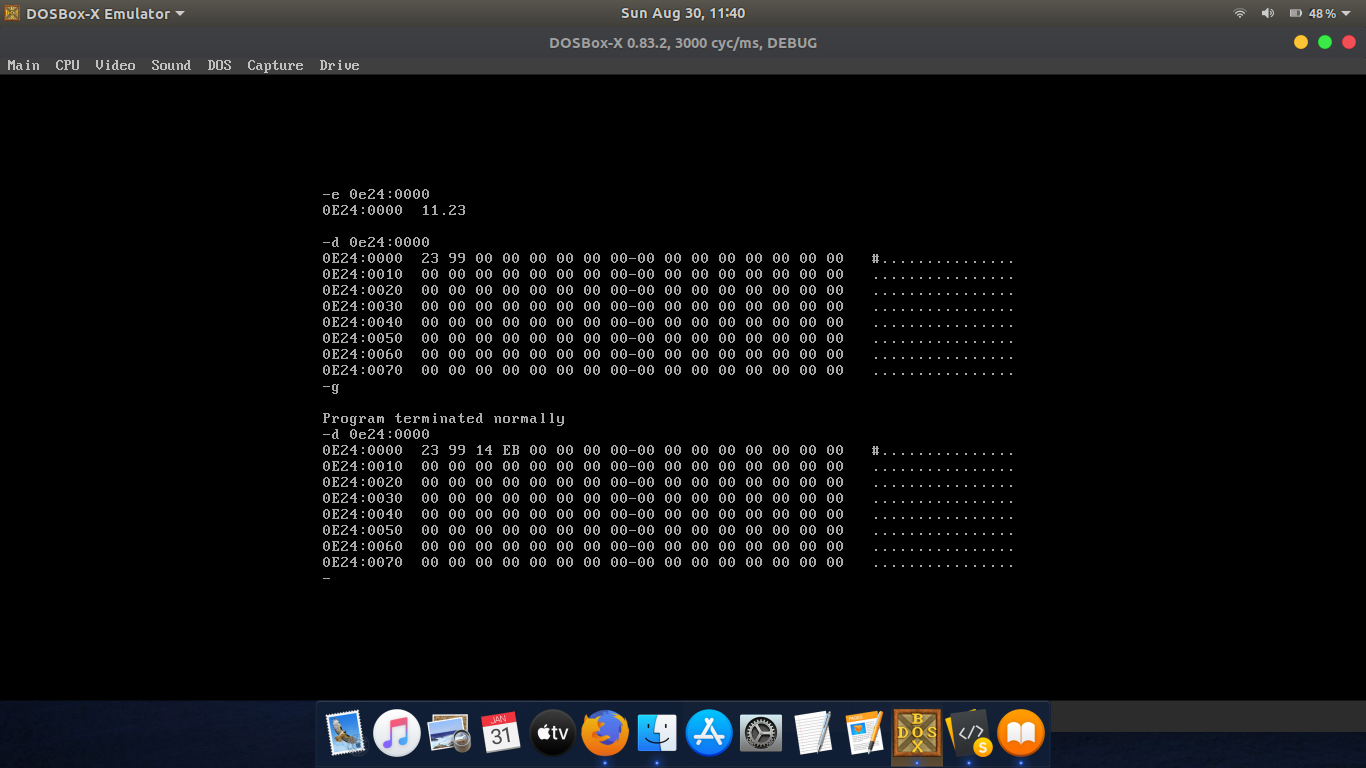
\includegraphics[trim = 100mm 70mm 100mm 80mm, clip, width = \textwidth]{Pics/Multiplication.png}
    \caption{ \textbf{Input:} \emph{opr1:} 23h, \emph{opr2:} 99h; 
              \textbf{Output:} \emph{Result:} EF 14h}
\end{figure}


%----------------------------------------------------------------------------------------------------------------------------------------
\newpage
\subsection*{\textbf{\underline{8 Bit Division}}}

\subsubsection*{\textbf{Algorithm:}}
\begin{itemize}
    \item Move the data segment to the AX register and then move it to the DS register.
\item  Now, set AH register to 00h and move first operand to AL register. (Since we can’t directly divide a 8 bit number by 8 bit number in
8086, we now make our dividend 16 bit by storing 00h in AH register and the 8-bit operand 1 in AL register).
\item  Move the second operand to the BL register.
\item  Now divide using DIV BL.( It will perform AX / BL. Because AH is 00h, what actually happens is the division of a 16 bit number by a
8 bit number).
\item  The quotient and remainder stored in AL and AH should be moved to QUOTIENT and REMAINDER respectively
\end{itemize}

\subsubsection*{\textbf{Program:}}
\begin{table}[h]
\centering\small
\resizebox{\columnwidth}{!}{
\begin{tabular}{|l|l|} 
\hline
\textbf{Program}                                                 & \textbf{Comments}                             \\ 
\hline
\hline
assume cs:code,ds:data                                           & Declare code and data segments                \\
\hline
data segment                                                     & Start of data segment                         \\
\hline 
opr1 db 11h                                                      & Define byte opr1 with hex value 11            \\
\hline
opr2 db 10h                                                      & Define byte opr2 with hex value 99            \\
\hline
resultq db 00H                                                   & Define byte resultq with hex value 00         \\
\hline
resultr db 00H                                                   & Define byte resultr with hex value 00         \\
\hline      
data ends                                                        & End of data segment                           \\
\hline
code segment                                                     & Start of code segment                         \\
\hline
org 0100h                                                        & Set preferred offset                          \\
\hline
start:~ mov ax,data                                              & Move data segment contents to AX register     \\ 
\hline
mov ds,ax                                                        & Move data in AX register to DS register       \\ 
\hline
mov al,opr1                                                      & Move contents of opr1 to AL register          \\ 
\hline
mov ah, 00H                                                      & Move hex value 00 to AH register              \\
\hline
mov bh,opr2                                                      & Move contents of opr2 to BH register          \\ 
\hline
div bh                                                           & AX = AL / BH                                  \\ 
\hline
here:~ mov resultq,ah                                            & Move contents of AH register to resultq       \\ 
\hline
mov resultr,al                                                   & Move contents of AL register to resultr       \\ 
\hline
int 21h                                                          & Request interrupt routine                     \\ 
\hline
code ends                                                        & End of code segment                           \\
\hline
end start                                                        &                                               \\
\hline
\end{tabular}
}
\end{table}

\newpage
\subsubsection*{\textbf{Input and Output:}}
\begin{figure}[h]
    \centering
    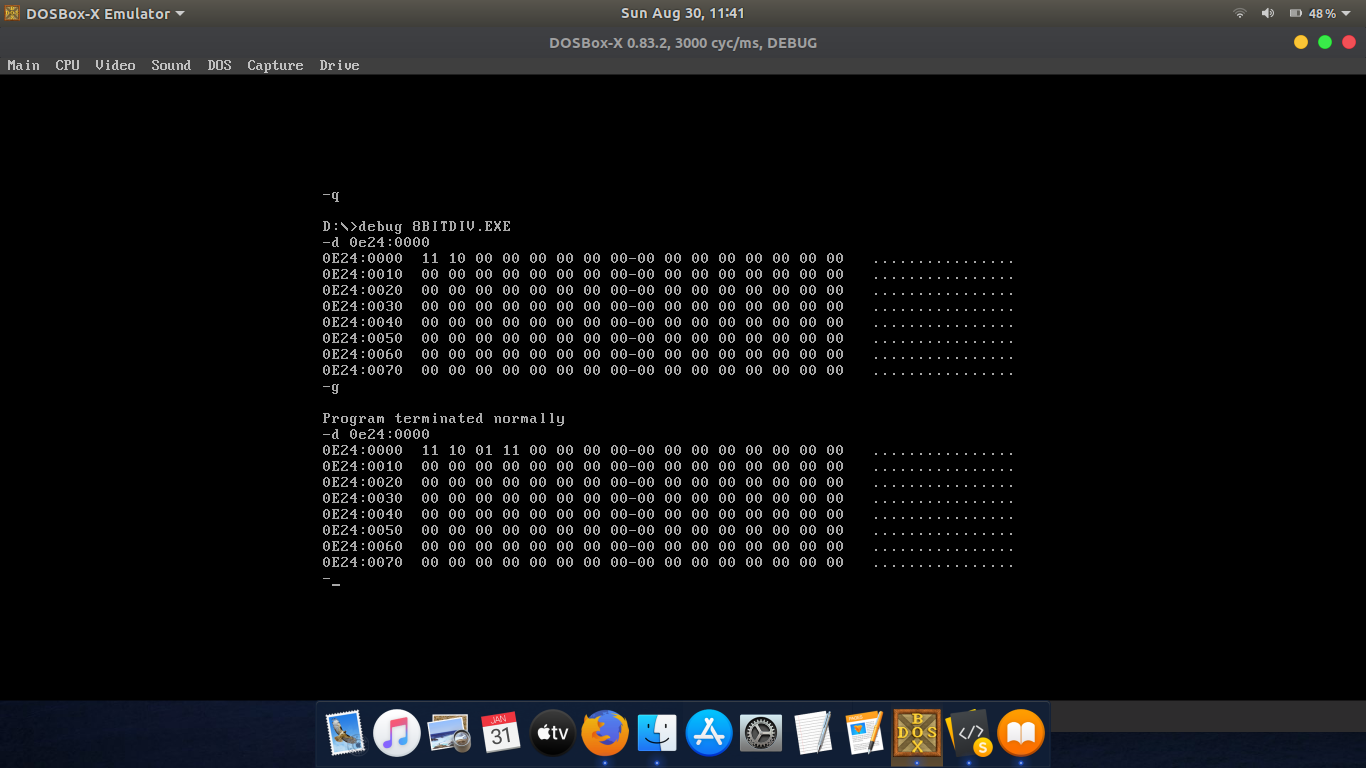
\includegraphics[trim = 100mm 70mm 100mm 80mm, clip, width = \textwidth]{Pics/Division.png}
    \caption{ \textbf{Input:} \emph{opr1:} 11h, \emph{opr2:} 10h; 
              \textbf{Output:} \emph{Quotient:} 01h, \emph{Remainder:} 11h}
\end{figure}

\hrule
\subsection*{\textbf{Result:}}
The 8086 programs were written to perform 8-bit arithmetic operations, and the results observed.
\end{flushleft}
\end{document}